\documentclass[11pt,letter]{article}
\usepackage[top=0.65in,bottom=0.9in,left=0.85in,right=0.85in]{geometry}

%\def\baselinestretch{1.25}
\def\baselinestretch{1.0}

\usepackage[greek, english]{babel}
\usepackage{multicol}

\usepackage{graphicx}
\usepackage[export]{adjustbox}


% The use of the times package forces the use of the type-1 times
% roman font, but the times roman font does not look nice.
% Besides the times roman font still does not print correctly on
% the dopy printer.
%\usepackage{times}


\usepackage{fancyhdr}
\usepackage{amsmath}
\usepackage{amssymb}
\usepackage{bm}
\usepackage{bbold}
\usepackage{parskip}
\usepackage{url}
\usepackage{xfrac}

\newcommand{\bv}[1]{\ensuremath{\bm{#1}}}
\newcommand{\vo}{\ensuremath{V_{0}}}
\newcommand{\bvo}{\ensuremath{\bv{V}_{0}}}
\newcommand{\er}{\ensuremath{E_{R}}}
\newcommand{\Lc}{\ensuremath{L_{\mathrm{c}}}}
\newcommand{\dsig}[1]{\ensuremath{ \frac{ d\,\sigma_{#1} }{d\,\Omega} }}
\newcommand{\dbl}{\ensuremath{ \uparrow\! \downarrow \, }}
\newcommand{\spup}{\ensuremath{ \uparrow }}
\newcommand{\spdn}{\ensuremath{ \downarrow}}
%\newcommand{\hhh}{\ensuremath{\left( \sfrac{1}{2}\,\sfrac{1}{2}\,\sfrac{1}{2}\right)  }}
\newcommand{\hhh}{\ensuremath{\left( \frac{1}{2}\,\frac{1}{2}\,\frac{1}{2}\right)  }}

\begin{document}


\section{ High-temperature series expansion for the single band Hubbard model }

In the vicinity of the atomic limit, where the tunneling between sites is small
compared to the on-site interactions,  the Hubbard model can be treated by
considering tunneling as a perturbation.   This treatment allows us to gain
insight into the different phases that the system can exhibit.  This section
follows closely after ~\cite{Henderson1992,Jordens2010}.   

We work in the grand canonical ensemble, so we include a global chemical potential
in the hamiltonian
\begin{equation}
\begin{split}
  H = &  
         \left( U\sum_{i} n_{i\spup} n_{i\spdn}  
         - \mu\sum_{i}( n_{i\spup} + n_{i\spdn} ) \right)
-t \sum_{ \langle ij \rangle, \sigma   } 
          a_{i\sigma}^{\dagger}a_{j\sigma} \\
   = &  H_{0} + H_{1} 
\end{split}
\end{equation}
For the unperturbed part, $H_{0}$, the grand canonical partition function is 
\begin{equation}
 Z_{0} = \text{Tr} e^{-\beta H_{0}} 
\end{equation}
Since the unperturbed part is a sum over sites, the partition function becomes
a product of the single site partition function: $Z_{0} = z_{0}^{k}$, for a
system with $k$ sites.  The single site partition function  is easy to
evaluate because the trace runs only over the four possible states in a single
site $\lbrace |0\rangle, |\spup\rangle, |\spdn\rangle, |\dbl\rangle\rbrace$.
\begin{equation}
 z_{0} = 1 + 2 e^{\beta\mu} + e^{\beta (2\mu-U)} = 1 + 2z + z^{2}u 
\end{equation}
where we have defined $z=e^{\beta\mu}$ and $u=e^{-\beta U }$.  Among the
relevant physical quantities that can be obtained are: the number of particles,
the number of double occupancies, and the entropy per site.  These are obtained
from the first derivatives of the grand canonical potential, $\Omega$
\begin{equation}
  \Omega = - \frac{\ln Z}{\beta}
\end{equation}
\begin{align}
  N &=  -\frac{\partial \Omega}{ \partial \mu }\\
  D &=  \frac{\partial \Omega}{ \partial U }  \\
  S &=  -\frac{\partial \Omega}{ \partial T} 
\end{align}
%\begin{gather}
%  N = -\frac{\partial \Omega}{ \partial \mu }  = z \frac{\partial}{\partial z} \ln Z\\
%  D = \frac{\partial \Omega}{ \partial U }  = u \frac{\partial}{\partial u} \ln Z\\
%  S = -\frac{\partial \Omega}{ \partial T}  = -\beta^{2}  \frac{\partial}{\partial \beta} \ln Z
%\end{gather}
Also, from the second derivatives of the grand potential one can obtain the
fluctuations in any of these quantities. 

For the full hamiltonian, the grand canonical partition function, $Z$, can be
expanded in a perturbation series~\cite{Henderson1992}: 
\begin{equation}
\begin{split}
  Z = & \text{Tr} e^{-\beta H}  \\
    = & Z_{0} \left[ 1 + 
        \sum_{n=1}^{\infty} (-1)^{n} 
        \int_{0}^{\beta} d\tau_{1} \int_{0}^{\tau_{1}} d\tau_{2} 
        \dotsm \int_{0}^{\tau_{n-1}} d\tau_{n} 
        \langle
              \tilde{H}_{1}(\tau_{1}) 
              \tilde{H}_{2}(\tau_{2})  \dotsm
              \tilde{H}_{n}(\tau_{n})  \rangle 
              \right] 
\end{split}
\end{equation} 
where the thermal expectation value inside the integral is taken with the
unperturbed hamiltonian
\begin{equation}
\langle A \rangle = \text{Tr} ( e^{\beta H_{0} } A ) / Z_{0} 
\end{equation}
and the tilde means that the operator is evaluated in the interaction picture,
for the imaginary time indicated: 
\begin{equation}
 \tilde{H}_{1}(\tau) = e^{\tau H_{0}} H_{1} e^{-\tau H_{0}} 
\end{equation}
Given the series expansion for $Z$, the grand potential is 
\begin{equation}
 -\beta \Omega = Z_{0} + 
        \sum_{n=1}^{\infty} (-1)^{n} 
        \int_{0}^{\beta} d\tau_{1} \int_{0}^{\tau_{1}} d\tau_{2} 
        \dotsm \int_{0}^{\tau_{n-1}} d\tau_{n} 
        \langle
              \tilde{H}_{1}(\tau_{1}) 
              \tilde{H}_{2}(\tau_{2})  \dotsm
              \tilde{H}_{n}(\tau_{n})  \rangle 
\end{equation}

One can see that the $n^{th}$ term in the expansion has $n$ copies of the
tunneling part of the hamiltonian.  Each  application of $H_{1}$ in the thermal
average results in a particle tunneling to a neighboring site, so we see that
there will be a contribution to the expansion only if, after $n$ tunneling
events, all the particles come back to their original sites.  As a direct
consequence, the first order term in the expansion vanishes.
The second order in the expansion corresponds to particles tunneling one site
over and then coming back.  Higher order terms can be represented by diagrams,
making it easier to keep track of them.  The contribution from orders up to
$n=9$ is shown in~\cite{Henderson1992}.  Here we will use up to the second
order term to illustrate the phases that appear in the system.  

The grand potential to second order is~\cite{Henderson1992,Jordens2010} 
\begin{equation}
-\beta \Omega_{2} = k \ln z_{0} + k \left( \frac{\beta t }{z_{0}} \right)^{2} m 
        \left( z + z^{3} u + 2z^{2} \frac{1-u}{\beta U} \right) 
\end{equation} 
where $m$ is the number of nearest neighbors for each lattice site, which in
the simple cubic case is $m=6$.  We see that the grand potential is
proportional to the number of lattice sites, $k$, so  all the
thermodynamic quantities will be expressed per lattice site.  The resulting
phase diagram is shown in Fig.~\ref{fig:highTphases} for a temperature
$T/t=2.5$.  
\begin{figure}
\centering 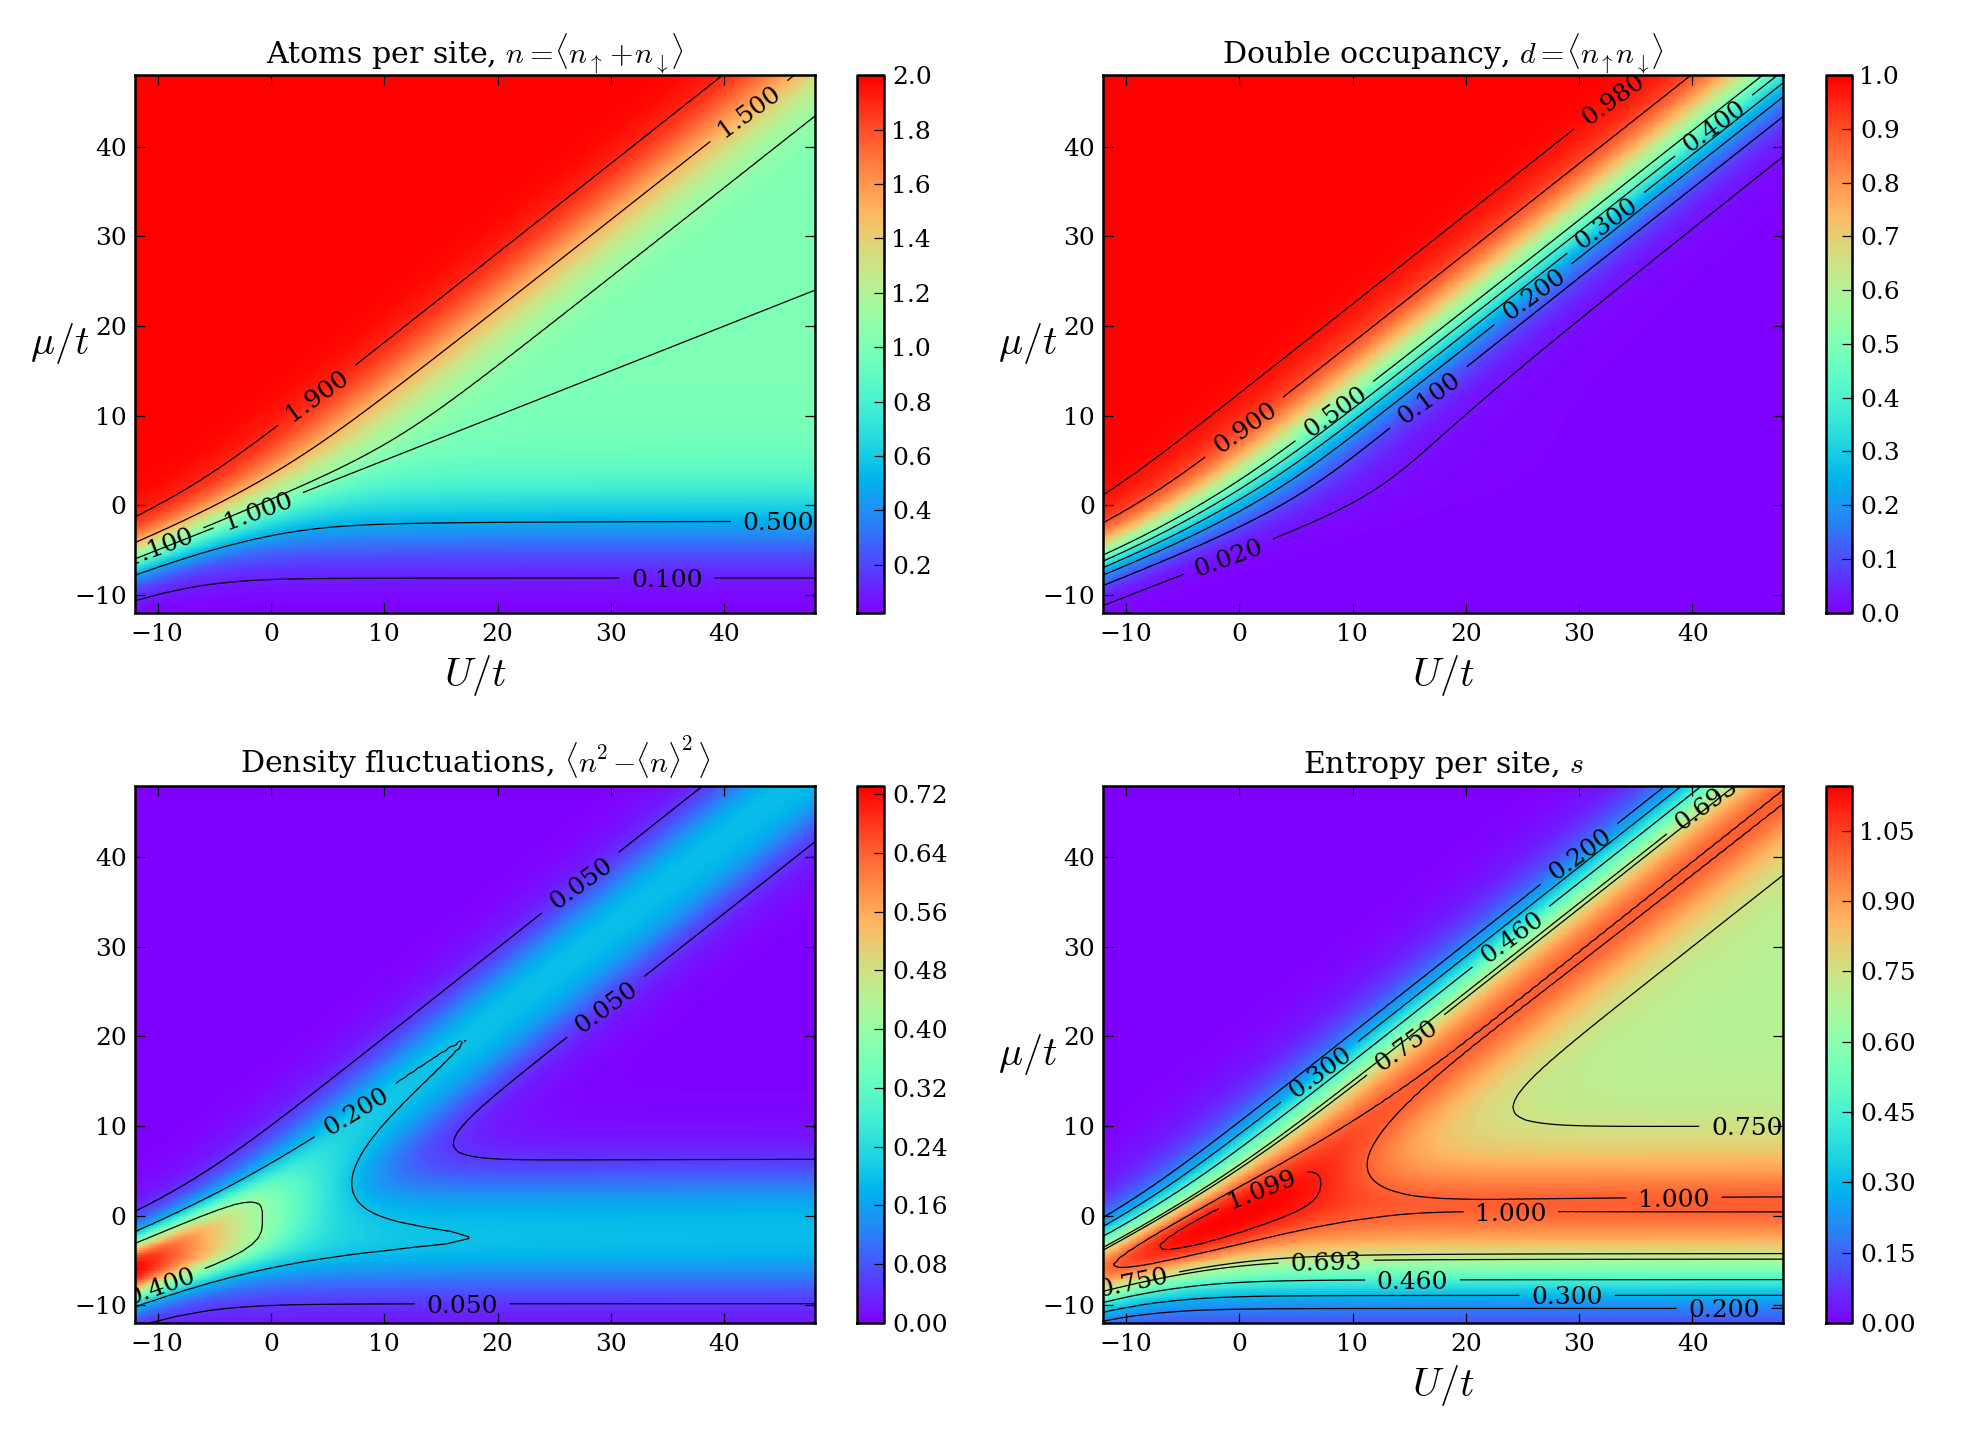
\includegraphics[width=\textwidth]{../HubbardPhaseDiagram_figures/HTSE_phasesT025.png}
\caption[High temperature phase diagram of the Fermi-Hubbard model]{\small High
temperature phase diagram of the Fermi-Hubbard model calculated using only up
to the second order in the perturbation series.  Temperature is given in units
of tunneling,  $T/t=2.5$. } \label{fig:highTphases}
\end{figure}

An important path along the phase diagram is the one corresponding to $\mu =
U/2$.  Along this line, referred to as half-filling, the density is always one
particle per site.  It can be shown~\cite{Scalettar:hubbard7} that the
phase diagram for the Hubbard model in a bipartite lattice\footnote{A bipartite
lattice consists of two sub-lattices $A,B$ such that all neighbors of $A$ are
in $B$ and vice-versa.~\cite{Scalettar:hubbard7}} is symmetric when the
chemical potential is reflected on the half-filling line.  The number of
particles per site $n \equiv \langle n_{\spup} + n_{\spdn}\rangle$, and the
local moment $\langle m^{2} \rangle  \equiv \langle (n_{\spup} - n_{\spdn})^{2}
\rangle $  as a function of chemical potential are given by 
\begin{equation}
\begin{split}  
  n( U/2 + \delta\mu ) =  & \  2 - n(  U/2 - \delta\mu ) \\
  \langle m^{2} \rangle ( U/2 + \delta\mu )= & 
      \  \langle m^{2} \rangle ( U/2 -  \delta\mu )
\end{split}
\end{equation}
The double occupancy, $d$, does not show the same symmetry in $\mu$, it is given by 
\begin{equation}
  d \equiv \langle n_{\spup}n_{\spdn} \rangle =  \frac{ n - \langle m^{2} \rangle} { 2 }
\end{equation}


The phase diagram obtained from the high temperature series expansion 
shows us the three insulating phases that exist in the Fermi-Hubbard model.
The vacuum, with zero particles per site is an insulating state,  and the Mott
insulator and band insulator have exactly one and two particles per site
respectively. The fluctuations in particle number vanish for the three
insulating states.  Also, the chemical potential shows a gap as a function of
the density, as shown in Fig.~\ref{fig:HighT_insulators}.  The gap in the
chemical potential around $n=1$ is known as the Mott gap.  
\begin{figure}
\centering 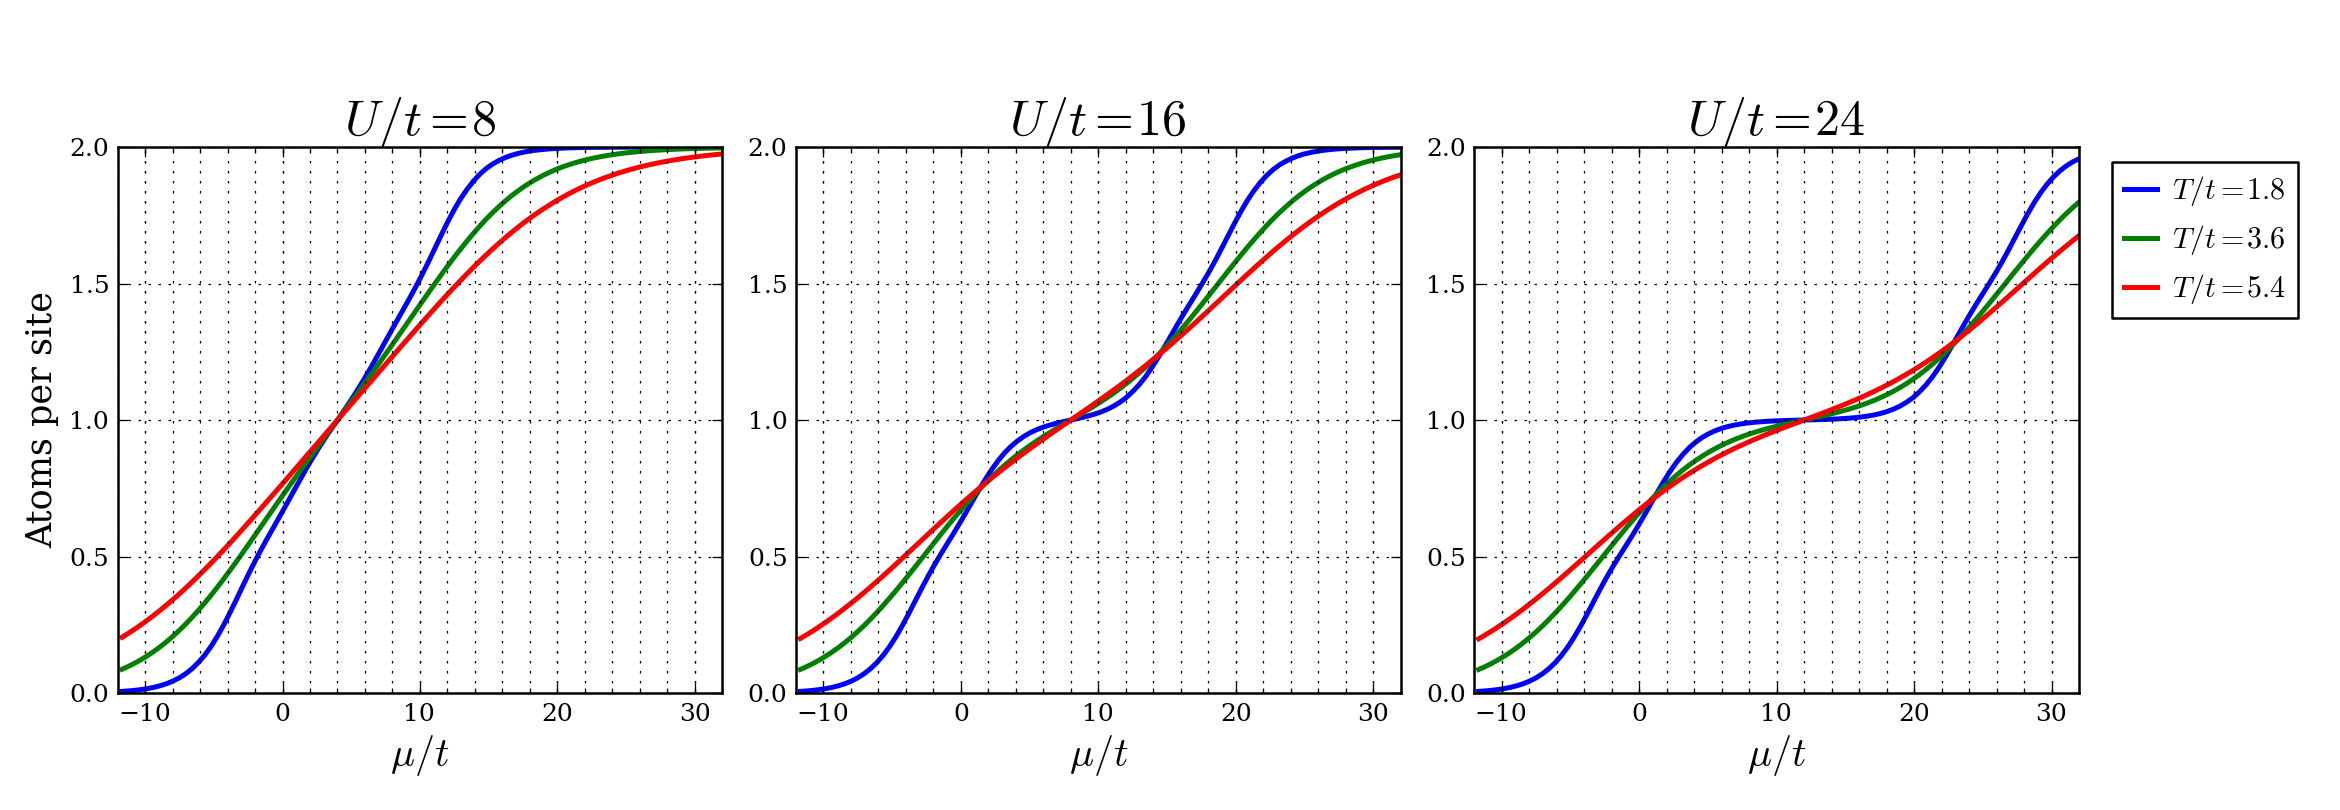
\includegraphics[width=\textwidth]{../HubbardPhaseDiagram_figures/HTSE_Density_U.png}
\caption[Density vs. chemical potential at various values of $U/t$]{\small
Density vs. chemical potential at various values of $U/t$ and for various
temperatures $T/t$. Calculated using only up to the second order in the
perturbation series. } \label{fig:HighT_insulators}
\end{figure}


\section{ Local density approximation }
\label{sec:lda}

In the local density approximation (LDA) we aim to establish local values for the
tunneling, the on-site interactions, and the chemical potential at each point in
our trap.  Using these local parameters, the phase diagram for the homogeneous
case can be used to calculate local thermodynamic quantities.  Integrals of the
local thermodynamic quantities can be directly linked to experimental
observables.  For example, the integral of the local density along an
observation axis yields the column density, which is measured directly via
in-situ phase-contrast imaging.   Also, an integral over all space of the local
double-occupancy yields the fraction of atoms in doubly-occupied sites.   This
can be measured experimentally by associating pairs of atoms into molecules (
using a magnetic field sweep across a Feshbach resonance), and then measuring
the number of molecules produced. 

In our experiment, the lattice has an underlying confining potential 
and, furthermore, the lattice depth varies as a function of position in the
trap.  Typically, the variation of lattice depth with position in the trap is
neglected when calculating the local parameters (tunneling, interactions and
chemical potential) because the waists of the lattice beams are
considerably
large,  $\gtrsim 150~\mu\mathrm{m}$.  In our setup, the beam waists are $\sim
45-50~\mu\mathrm{m}$ and we have to consider the variation of the lattice depth
in the region that is sampled by the atoms. 

At each point $\bv{r}$, the depth of the lattice can be different in the three
orthogonal directions.  The lattice depth, $V_{0}$, is then a set of three
numbers $V_{0}(\bv{r}) \equiv \lbrace V_{0x}(\bv{r}), V_{0y}(\bv{r}),
V_{0z}(\bv{r}) \rbrace$.  The hamiltonian for an atom moving in a simple cubic
lattice is separable in the three spatial coordinates, so having three
different lattice depths poses no problem in finding the 3D band structure, and
the 3D Wannier states of the local lattice potential.  On the other hand, it is
more complicated to go through the calculation of the phase diagram with three
different tunneling matrix elements; instead, for each $\bv{r}$, we use the
average tunneling matrix element as the input for the phase diagram, in order
to calculate the local thermodynamic quantities.  To calculate the local
on-site interactions we use integrals of the 3D Wannier states,  which are
simply products of 1D Wannier states for each of the three orthogonal
directions. 

We obtain the local chemical potential at each point in the trap as  
\begin{equation}
 \mu(\bv{r}) = \mu - E_{0}(\bv{r}) 
\end{equation}
The quantity $E_{0}(\bv{r})$ is a combination of the confining potential that
envelopes the purely sinusoidal lattice potential and the zero of energy in the
Fermi-Hubbard hamiltonian.   In the Fermi-Hubbard hamiltonian, the kinetic
energy for motion in the lattice potential is 
\begin{equation}
-t \sum_{ \langle ij \rangle, \sigma   } 
          a_{i\sigma}^{\dagger}a_{j\sigma} 
\end{equation} 
This sum is restricted over nearest neighbors.  In the microscopic derivation
of the Fermi-Hubbard model there are also terms that involve a single site,
but they are typically discarded because they only add a constant energy given
by 
\begin{equation}
-\sum_{i\,\sigma} t_{ii} 
          a_{i\sigma}^{\dagger}a_{i \sigma}  = - t_{0} \sum_{i\,\sigma} n_{i\sigma} 
\end{equation}
where 
\begin{equation}
 - t_{0} = \left( 
          \frac{1}{L} \sum_{q_{x}} E_{q_x}^{\text{\tiny 1D}} 
         + \frac{1}{L} \sum_{q_{y}} E_{q_y}^{\text{\tiny 1D}} 
         + \frac{1}{L} \sum_{q_{z}} E_{q_z}^{\text{\tiny 1D}} 
    \right)
\end{equation}
It becomes clear that $-t_{0}$ is the average energy of the lowest band in 3D,
which can be readily obtained given the set of three lattice depths along each
of the orthogonal axes.   

In the most common use of the LDA in a trap, the local
chemical potential is given by 
\begin{equation}
 \mu(\bv{r}) = \mu - V_{\text{trap}}(\bv{r}) 
\end{equation}
but we have seen here that to apply the local density to the lattice potential
we need to consider the local band structure of the lattice, as well as the
confining potential that envelopes the purely sinusoidal lattice potential.  We
have aggregated those two terms in the quantity $E_{0}(\bv{r})$.  We note here
that, for implementations with large lattice beam waists, the lattice depth can
be taken as a constant over the region occupied by the atoms.  This means that
the local band structure does not vary over the sample, and the quantity
$E_{0}(\bv{r})$ can be replaced by only the confining potential.  This is the
typical way in which LDA is applied to a
lattice~\cite{DeLeo2008,DeLeo2011,Gorelik2010,Fuchs2011}, except for the
treatment in~\cite{Mathy2012} which takes into account the length scales set by
the waists of the lattice beams. 

We show in Fig.~\ref{fig:illustrate_lda}  an illustration of the application of
the LDA to a compensated lattice potential.   
\begin{figure}
 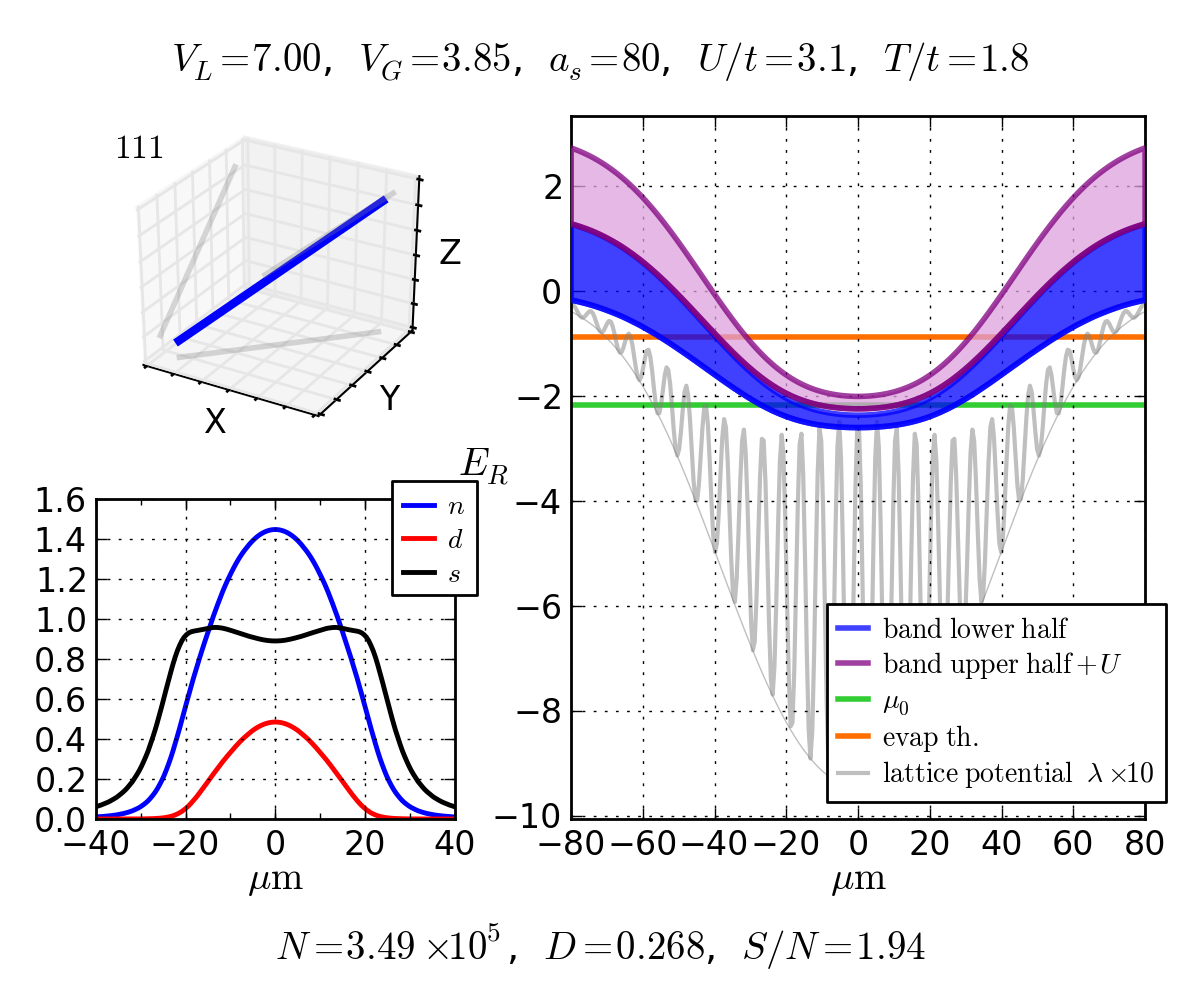
\includegraphics[width=0.5\textwidth]{../Ut_Comp/T00/111_as0080.png}
 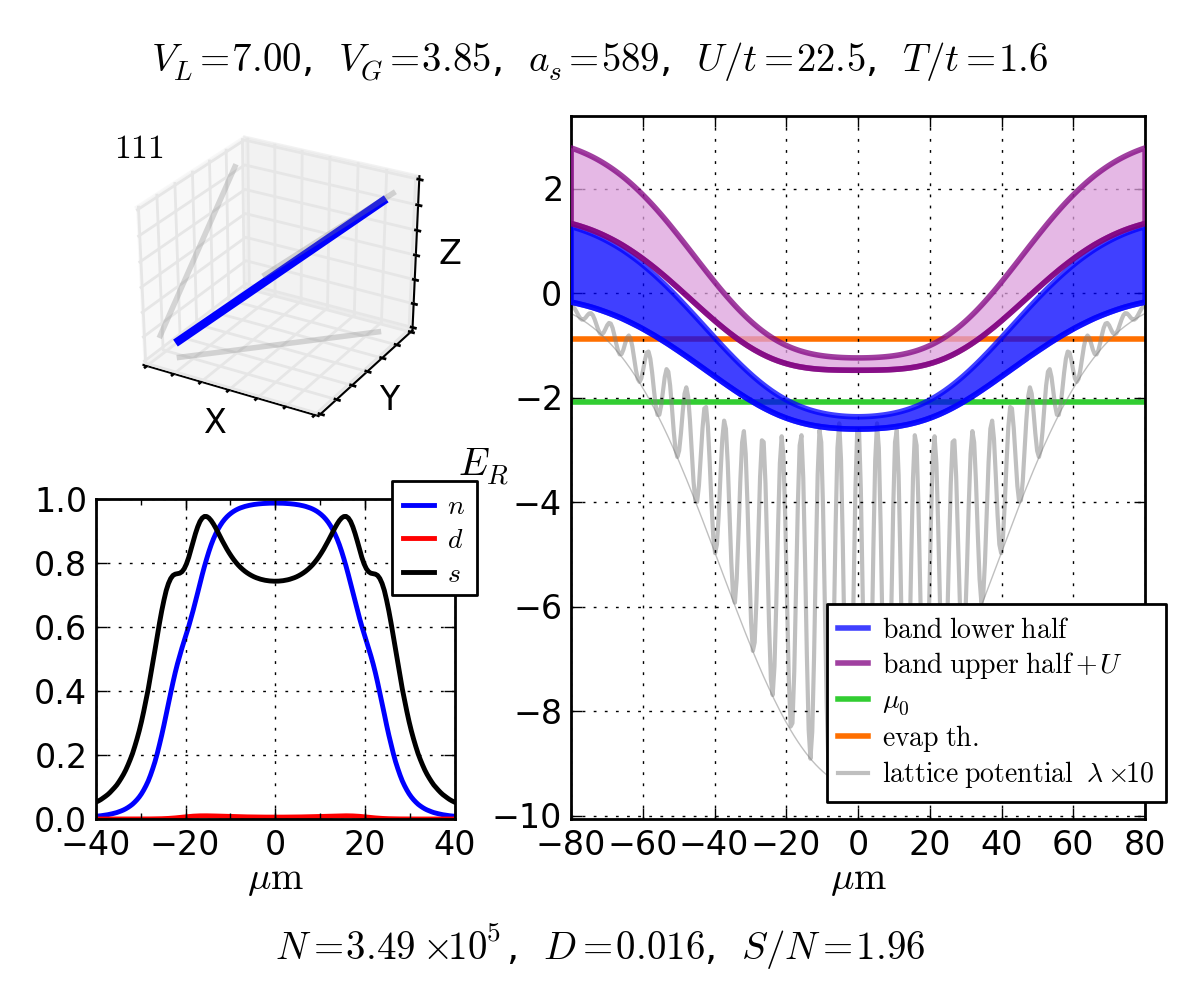
\includegraphics[width=0.5\textwidth]{../Ut_Comp/T00/111_as0589.png}
\caption[Local density approximation in a compensated lattice potential]{\small
Illustration of the local density approximation in a compensated lattice
potential.  The left panel shows a situation with small interactions, obtained
by setting a scattering length of 80 $a_{0}$. For the right panel the
scattering length is 589 $a_{0}$.  See the text for a detailed explanation. } 
\label{fig:illustrate_lda}
\end{figure}
On the left the scattering length is 80 $a_{0}$,  which corresponds to a
relatively small $U/t=3.1$ at the center of the lattice.   On the right, the
scattering length is 589 $a_{0}$, which corresponds to $U/t=22.5$ at the
center.   All of the lines plots are along the 111 direction,  as illustrated
on the top left inset in each panel.  

The larger plot on the right of each panel shows the 3D band structure, the
global chemical potential, the lattice potential, and the threshold for
evaporation.  The sinusoidal lattice potential is enveloped at the bottom by an
overall confinement that results from the lattice beams plus the contribution
from the green compensation beams.   The lattice modulation is shown, with the
wavelength scaled $\times10$ for clarity.  The depth of the modulation
corresponds to the smallest of the three lattice depths $V_{0x}(\bv{r})$,
$V_{0y}(\bv{r})$, $V_{0z}(\bv{r})$ at a given point, $\bv{r}$, in the trap. 
Along the 111 direction we have $V_{0x} = V_{0y} = V_{0z}$. 

The 3D band structure is shown with the shaded blue and purple areas.  The blue
area shows the lower half of the band.  The bottom of the blue area corresponds
to the lowest available single particle energy level.  The top of the blue area
corresponds to the average energy of the lowest band,  which is exactly the
quantity $E_{0}(\bv{r})$ that we defined above.   The local chemical potential
is measured with respect to $E_{0}(\bv{r})$.  The purple area shows the upper
half of the band plus the contribution from the on-site interactions.  The
spacing between $E_{0}(\bv{r})$ and the bottom of the purple band corresponds
to the Mott gap at zero temperature. 

On the bottom left of each panel in Fig.~\ref{fig:illustrate_lda} we show the
local thermodynamic quantities, namely the number of particles per site ($n$),
the double-occupancy per site ($d$), and the entropy per site ($s$).  On the
left, at 80 $a_{0}$, we see that the interactions are not strong enough to have
a Mott insulating state, and the density at the center is above one particle
per site.  On the right, at 589 $a_{0}$ the density is capped at one per site
at the center of the trap due to the large value of the on-site interactions.  

The orange line, which is labeled as the evaporation threshold, is better
understood if we make a line plot along one of the lattice directions, for
instance 100. This is shown in Fig.~\ref{fig:illustrate_evap}. 
\begin{figure}
\centering 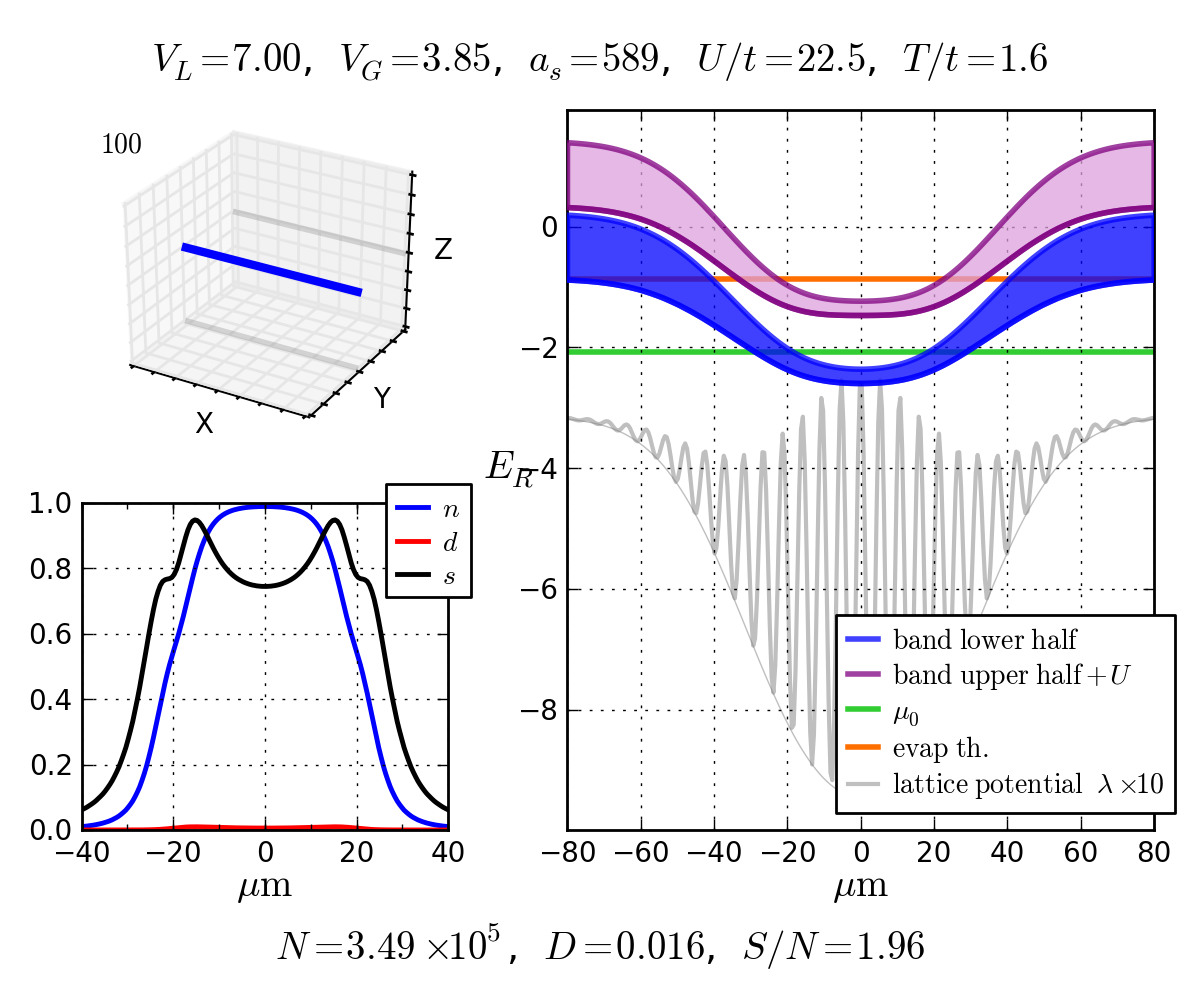
\includegraphics[width=0.5\textwidth]{../Ut_Comp/100_as0589.png}
\caption[Evaporation threshold in a compensated lattice potential]{\small
Illustration of the local density approximation in a compensated lattice
potential. Line plot along 100 for a scattering length of 589 $a_{0}$. See the
text for a detailed explanation. } \label{fig:illustrate_evap}
\end{figure}
The evaporation threshold is the energy that a particle needs to escape along
one lattice beam.  If it has enough energy, the particle can escape the central
part of the trap by tunneling along a lattice direction.   The situation is
slightly different than in a non-lattice potential, since the velocity of
escape will be reduced due to the presence of the lattice, and furthermore the
particle may Bragg scatter off of the lattice and be kicked back towards the
center of the trap. 

\subsection{Validity of the local density approximation} 

The LDA breaks down at low temperatures, where long
range correlations become important for the description of the system.   In the
high temperature series expansion, the correct solution at lower temperatures
can only be obtained if sufficient orders in the series are considered.  We
recall that the $n^{\text{th}}$ term in the series can be associated to a
particle tunneling $n$ times and returning to its original position.  That
means that the particle must explore a region of size $a\sqrt{n}$, where $a$ is
the lattice spacing.   If the values of the local parameters ($t$, $U$, and
$\mu$) vary considerably over  $a\sqrt{n}$, then the applicability of the local
density approximation for the series solution stops making sense.   This will
inevitably happen at low enough temperatures,  where long range correlations
start to develop in the system.    The break-down of LDA makes it very
challenging to consider inhomogeneous systems at low temperatures.   At the
same time,  the most interesting physics is associated with the appearance of
long range order and the resulting phase transitions that occur at low enough
temperatures.  The prime example is the transition from a Mott insulator to an
antiferromagnetic Mott insulator, which is expected to happen at a temperature
of around $T/t \sim 0.3-0.4$~\cite{Staudt2000,Kent2005,Fuchs2011,Paiva2011}. 

\section{Experimental measurement of the double-occupancy and comparison with the LDA}

In our experiment we can measure double-occupancies by making use of the narrow
Feshbach resonance at 543 G.  The scattering length as a function of magnetic
field is shown in Fig.~\ref{fig:scattlen_bfield}.
\begin{figure} \centering
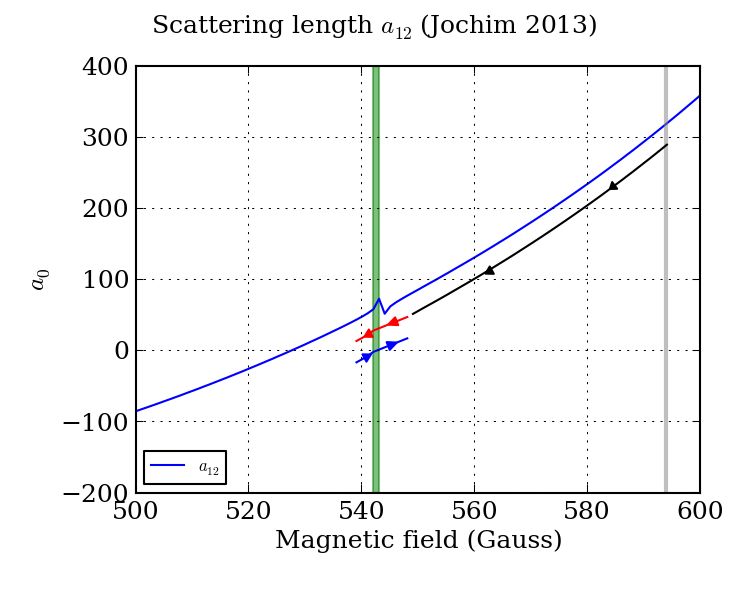
\includegraphics[width=0.5\textwidth]{../2_Data/ajochim_plot.png}
\caption[Scattering length as a function of magnetic field]{\small
Scattering length as a function of magnetic field in the region relevant for
simulation of the repulsive Fermi-Hubbard model.   The scattering length data
is obtained from~\cite{Zurn2013}.  The vertical green line marks the position
of the narrow Feshbach resonance.   The arrows show the magnetic field sweeps
that are used to go from the initial value of the scattering length to a value
approaching the narrow resonance (black), then sweep across the resonance to
associate doubly-occupied sites into molecules (red), and then back across the
resonance do dissociate the molecules back into atom pairs (blue).    
} \label{fig:scattlen_bfield} 
\end{figure}
We perform our lattice loading ramps as usual, reaching a lattice depth of
$7\,E_{R}$ with a green compensating potential of $4\,E_{R}$.  The scattering
length is set to the desired value during the lattice loading ramps.   After
the final parameters are reached, the lattice depth is suddenly increased to
$50\,E_{R}$ (at the center of the trap) in order to prevent any further motion of
particles.  After this is done, we first ramp the magnetic field in 8 ms down
to 80 $a_{0}$; from there we go across the resonance to 61 $a_{0}$ in
24 ms.  Pairs of atoms in doubly occupied sites are associated to create
molecules when the magnetic field is ramped across the resonance.  The
resulting molecules are far detuned with respect to the free atoms,
so we can take an in-situ phase contrast image to reveal the distribution of
atoms in singly occupied sites.  

At this point we can also opt to blow away the atoms using a resonant
light pulse, and then sweep the magnetic field back across the resonance
to dissociate the molecules.  In this way we can directly image the
in-situ distribution of doubly-occupied sites.   At the moment we do not
have the data for the direct double-occupancy measurement. We were
technically limited by our inability to blow away single atoms in both
of the spin states in a time small compared to the lifetime of the
molecules.    Even though we are at $50\,E_{R}$ we observe a finite
lifetime of the molecules which depends on the number of atoms in singly
occupied sites.   We believe, as was suggested in~\cite{Thalhammer2006},
that the fast molecular decay is due to atoms that tunnel to a site that
has a molecule and inelastically collide with it.  

The data that we have at the moment consists of pictures of the in-situ density
distribution taken at three different times in the sequence: 
\begin{enumerate}
\item Right before locking the lattice to $50\,E_{R}$.  Lattice depth is
$7\,E_{R}$.  
\item Right after locking the lattice to $50\,E_{R}$.  
\item Right after performing the magnetic field sweep that associates
doubly-occupied site into molecules. 
\end{enumerate}

With this data, we integrate the in-situ density distributions to obtain the
total fraction of atoms in singly occupied sites.  The complement of this is
the total fraction of atoms in doubly occupied sites, $D$.   The image of the
atoms in singly occupied sites is taken only a few milliseconds after crossing
the Feshbach resonance.  This should minimize systematic effects, due to atom
losses from inelastic collisions with molecules.   In any case, the measurement
should be strictly considered as a lower bound on the number of atoms in singly
occupied sites.   The complement, $D$, is then an upper bound on the total
fraction of atoms in doubly-occupied sites. 

Using the LDA,
as shown in Section~\ref{sec:lda}, we can obtain local values of the
thermodynamic quantities at any position in our trap.   We integrate the local
double-occupancy to find $D$, which can then be compared to the experimentally
determined quantity. The results are shown in
Fig.~\ref{fig:doubleocc_Comp_data}.  
\begin{figure} \centering
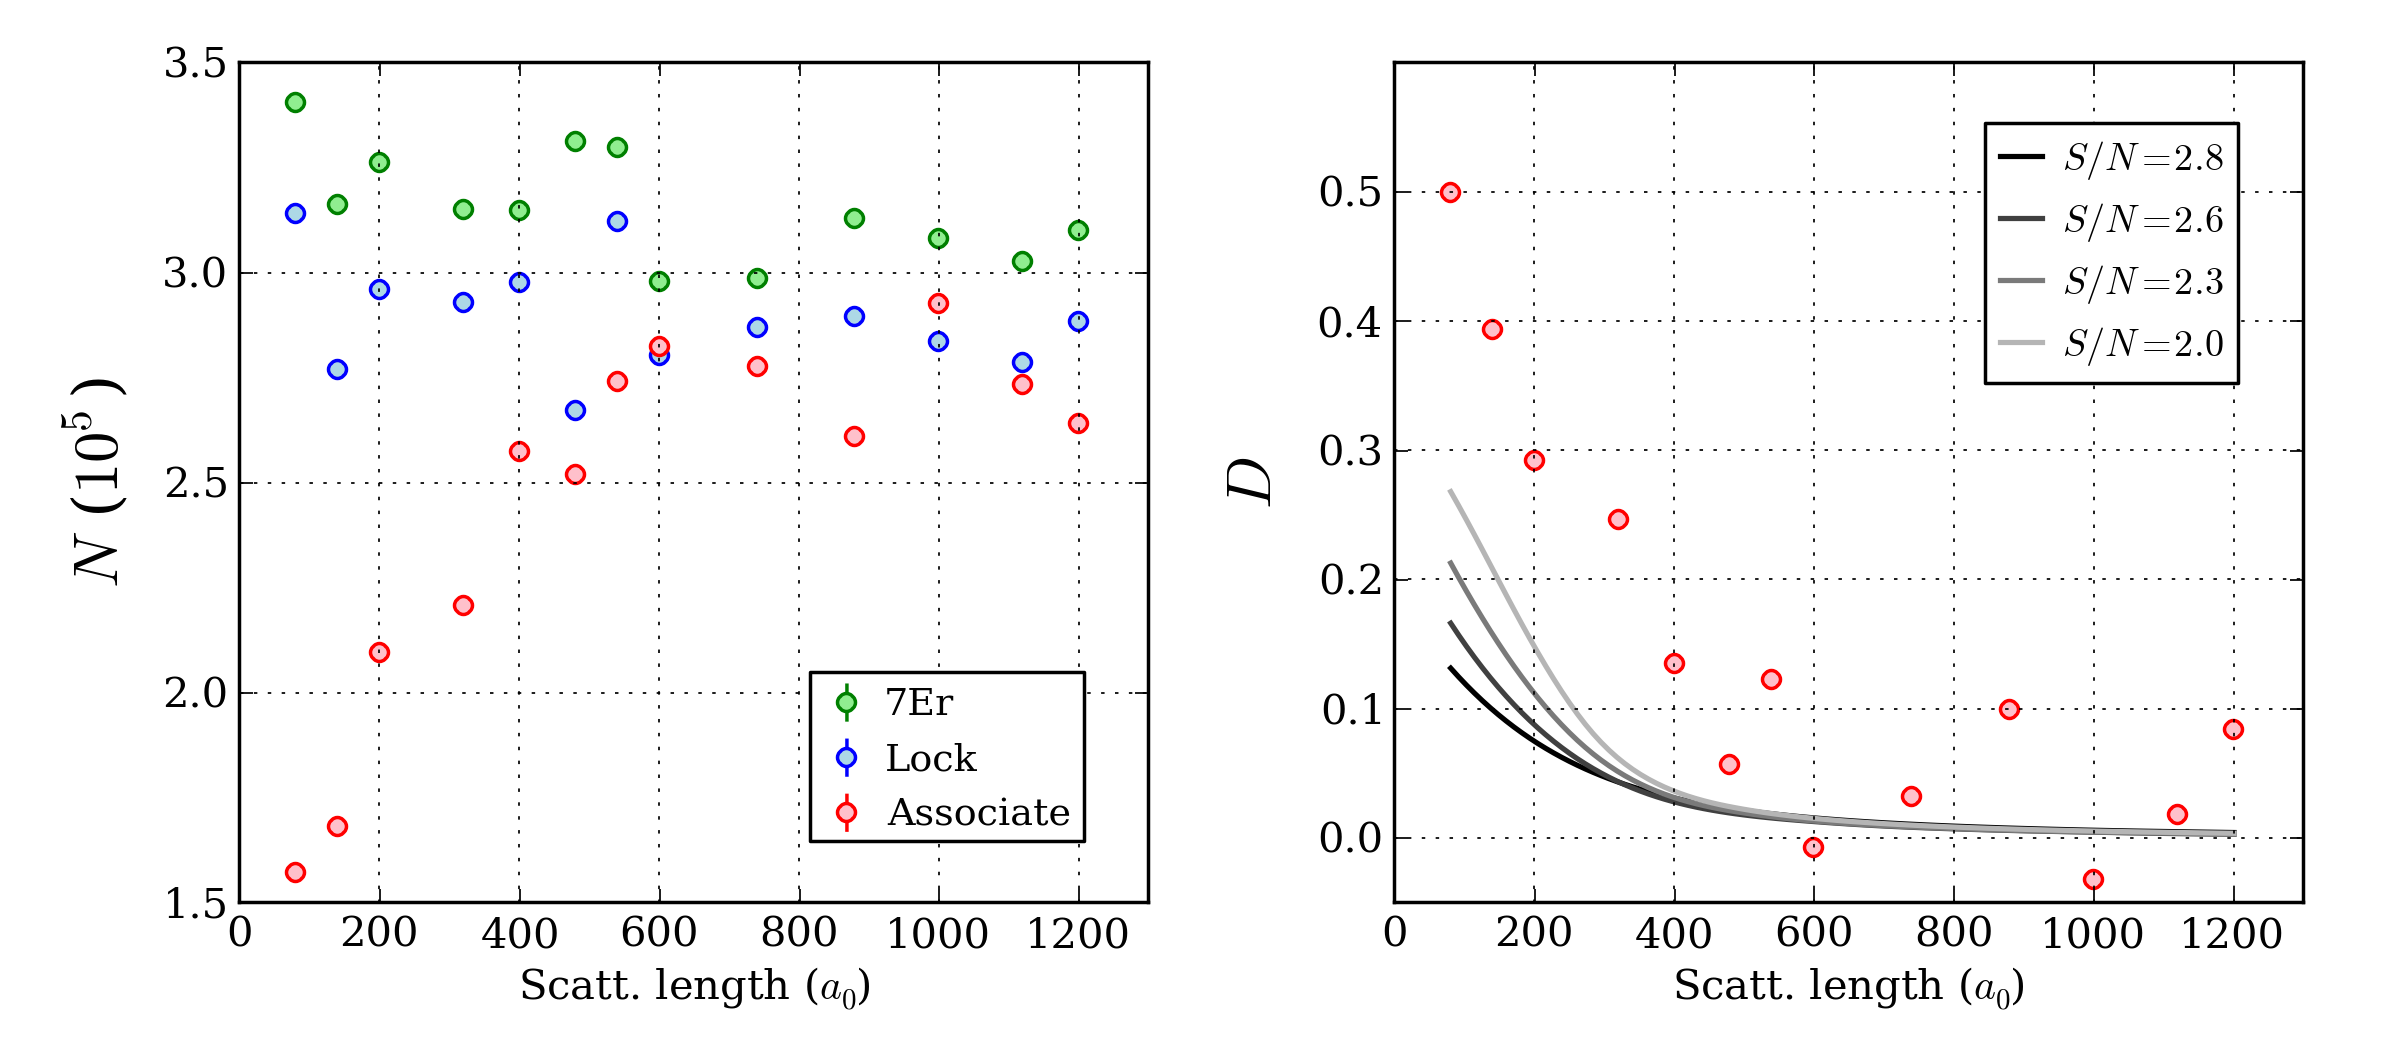
\includegraphics[width=\textwidth]{../Ut_Comp/doubleocc_.png}
\caption[Measurement of the fraction of atoms in doubly occupied sites as a
function of scattering length. ]{\small Measurement of the fraction of atoms in
doubly occupied sites as a function of scattering length.  The left panel shows
the atom number measured in-situ (green points) in a  $(7.5, 7.5, 8.5) \,E_{R}$
lattice (Note: We were aiming for a $7\,E_{R}$ lattice but we had a bad
calibration of the lattice depths, see Section~\ref{sec:disclaimer}), at
$50\,E_{R}$ after locking the lattice (blue points), and after associating
atoms in doubly occupied sites to form molecules (red).  The right panel shows
the fraction of atoms in doubly occupied sites and the results obtained from
the LDA at various values of total entropy per particle. (In this figure each
point is from a single experimental run.  We plan to take more data so that we
can do a better average at each point and include an error bar.)  }
\label{fig:doubleocc_Comp_data} 
\end{figure}

We see that the fraction of atoms in doubly-occupied sites that we observe is
larger than what is expected from the LDA and the high temperature series
expansion to second order.  In the LDA, for a given $U/t$, $D$ increases for
lower entropy.  This is contrary to intuition, as one expects double
occupancies to be thermally activated in the system.  In the trapped system, the
increase in $D$ with entropy is a consequence of the reduction of the central
density at higher entropy.  This point is made
in~\cite{Jordens2010b}, where a detailed study of the double-occupancy as a
function of  characteristic filling\footnote{Characteristic filling is
$\rho=N/N_{0}$ where $N_{0}$ is the number of atoms per spin that produces half
filling in the center of the trap at zero temperature and without
interactions~\cite{Jordens2010b}.} and interaction strength was performed with
$^{40}$K atoms in a simple cubic lattice.   

It is also pointed out in~\cite{Gorelik2010} that, even for the homogeneous
model, the double-occupancy can be enhanced in the antiferromagnetic core since
each atom is surrounded by only opposite spins.  An atom can lower its energy
in a second order process by virtually hopping to any of the nearest neighbors.
In contrast, in the paramagnetic state, half of the neighbors are of the same
spin, so tunneling to those sites is forbidden by the Pauli principle.  It is
shown in~\cite{Gorelik2010} that such an enhancement is significant only
for $U/t > 9$, so it cannot be really related to the large value of $D$ that we
observe for the smaller values of $U/t$. 

An interesting result shown in~\cite{Gorelik2010} is related to the column
integral of the local double occupancies.  It is shown there that the
double-occupancy profile somewhat resembles the shape of the antiferromagnetic
core, and thus could be used as an indicator of its presence.  

Other experiments typically perform double-occupancy measurements in
time-of-flight, however we have the possibility of accessing the in-situ
double-occupancy using phase-contrast imaging.  
%This is a consequence of using
%a closed-channel dominated resonance to associate atom pairs into molecules,
%which puts the molecules conveniently out of reach for a laser resonant with
%free atoms.  
An in-situ measurement of the double-occupancy would involve
associating atom pairs, then blowing away free atoms with a resonant pulse,
then dissociating the remaining molecules and imaging them using in-situ
phase-contrast imaging.  A technical limitation forced us to wait about 70 ms
in between blow away pulses for atoms in states $|1\rangle$ and $|2\rangle$.
This wait is too long given the short lifetime of the molecules in the lattice.
We have since overcome the time limitation and we can blow away the two states
simultaneously (but we have not taken the data yet).  This should allow us to
circumvent the short lifetime of the molecules and take in-situ data for the
double-occupancy.   

Furthermore the direct measurement of the double-occupancy would allow us to put
a lower bound on $D$,  which would address the possibility that the larger $D$
that we observe is due to a systematic overestimation.  


\section{ Latest Bragg scattering data as a function of scattering length}

Lately we have been trying to get final data on the Bragg scattering signal as
a function of the scattering length.  Our main issue continues to be the
stability and reproducibility in aligning the compensated lattice potential.  

The data that we have taken so far is shown in Fig.~\ref{fig:utdata}.  We do
our usual lattice loading ramps, then we suddenly ramp up the lattice to
$20\,E_{R}$ and probe with the Bragg beam.   We tried using a $50\,E_{R}$
lattice lock, but the Bragg signal was not as strong we suspect that it has to
do with the speed of the lock ramps.  Doing any further studies on that
variable is expensive in time, so we decided to stick to the $20\,E_{R}$ ramp
which happens in about 150\,$\mu$s (limited by our intensity stabilization
circuitry).  The main point that stands out is that we observe the largest AFM
correlations in a $U/t$ region where the fraction of atoms in doubly occupied
sites is still considerably large.  We are extending this question to our
theory collaborators in hope of a better understanding of what is going on.  
\begin{figure} \centering
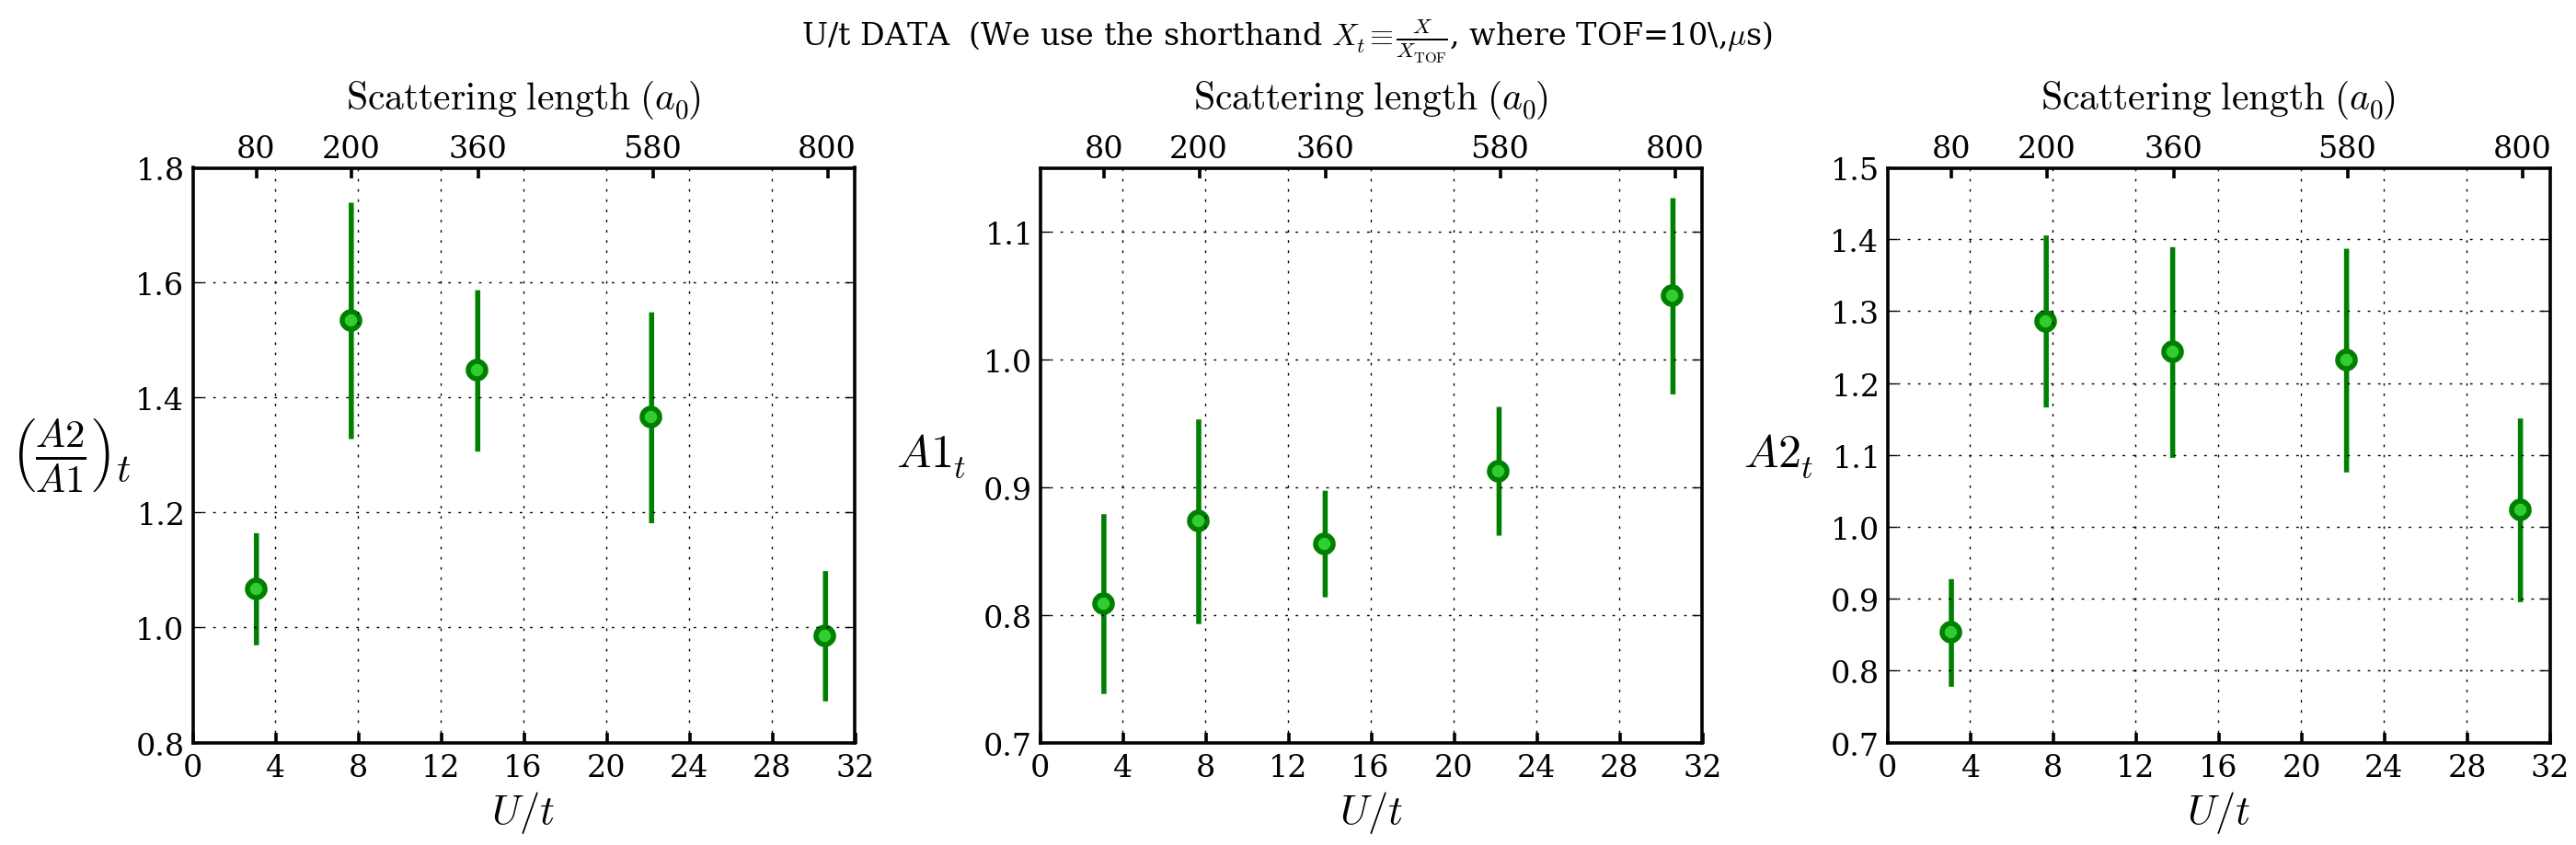
\includegraphics[width=\textwidth]{../Ut_Comp/udata_average_Fancy.png}
\caption[\hhh\ Bragg scattering as a
function of scattering length. ]{\small \hhh\ Bragg scattering as a function of scattering length. } \label{fig:utdata} 
\end{figure}

Below we enumerate a few points:
\begin{enumerate}
 \item  The best indicator of AFM correlations should be in $A2_{t}$. 
    \begin{itemize}
    \item  However, this measure is also susceptible to any suppression of light
scattering due to the presence of double occupancies.  This may have something
to do with the $<1$ point at 80 $a_{0}$ for $A2_{t}$.  For more information on the suppression of light scattering due to double occupancies see Sec.~\ref{sec:suppression}.
    \item A technical problem with $A2_{t}$ is that in-situ shots and TOF shots
come from different experimental runs.  So this measure has added noise due to
atom number variations and probe intensity variations from shot to shot .  
     \end{itemize}
 \item  There is suppression of light scattering in $A1_{t}$.   
    \begin{itemize}
    \item One may suggest that this comes 
from a strong AFM Bragg scattering signal that we may be missing due to bad
placing of the input Bragg beam or the $A2$ camera.  We have attempted to vary
the input Bragg beam angle and the $A2$ camera angle to try to find a steep
slope on $A2_{t}$ but we have found nothing.  This makes us believe that the
angular distribution of Bragg scattering is broad (as we learned from our
previous rocking curve data) and that the suppression observed here in $A1_{t}$
is related to the double occupancies at the lower scattering lengths.  
    \end{itemize}
\item  The signals that we obtain are noisy because we do not have many photons
reaching our cameras.  
    \begin{itemize}
       \item A nice feature of $A2/A1$ is that noise due to shot-to-shot atom
number and probe variations is canceled out because $A2$ and $A1$ can be
recorded simultaneously for every shot.  
    \end{itemize}
\end{enumerate}

\subsection{Suppression of light scattering due to the presence of double-occupancies}
\label{sec:suppression} 

A few weeks ago we studied briefly the suppression of light scattering due to
the presence of double-occupancies.  To do this, we created sample with only
doubly-occupied sites. This was done by sweeping through the Feshbach
resonance, blowing away singly occupied sites and then dissociating the
resulting molecules.   At a lattice depth of $50\,E_{R}$, we observed a
suppression in the scattered light in the in-situ pictures for a probe light
detuning in between the two hyperfine states.  This is shown in
Fig.~\ref{fig:lightsupress}.
 \begin{figure} \centering
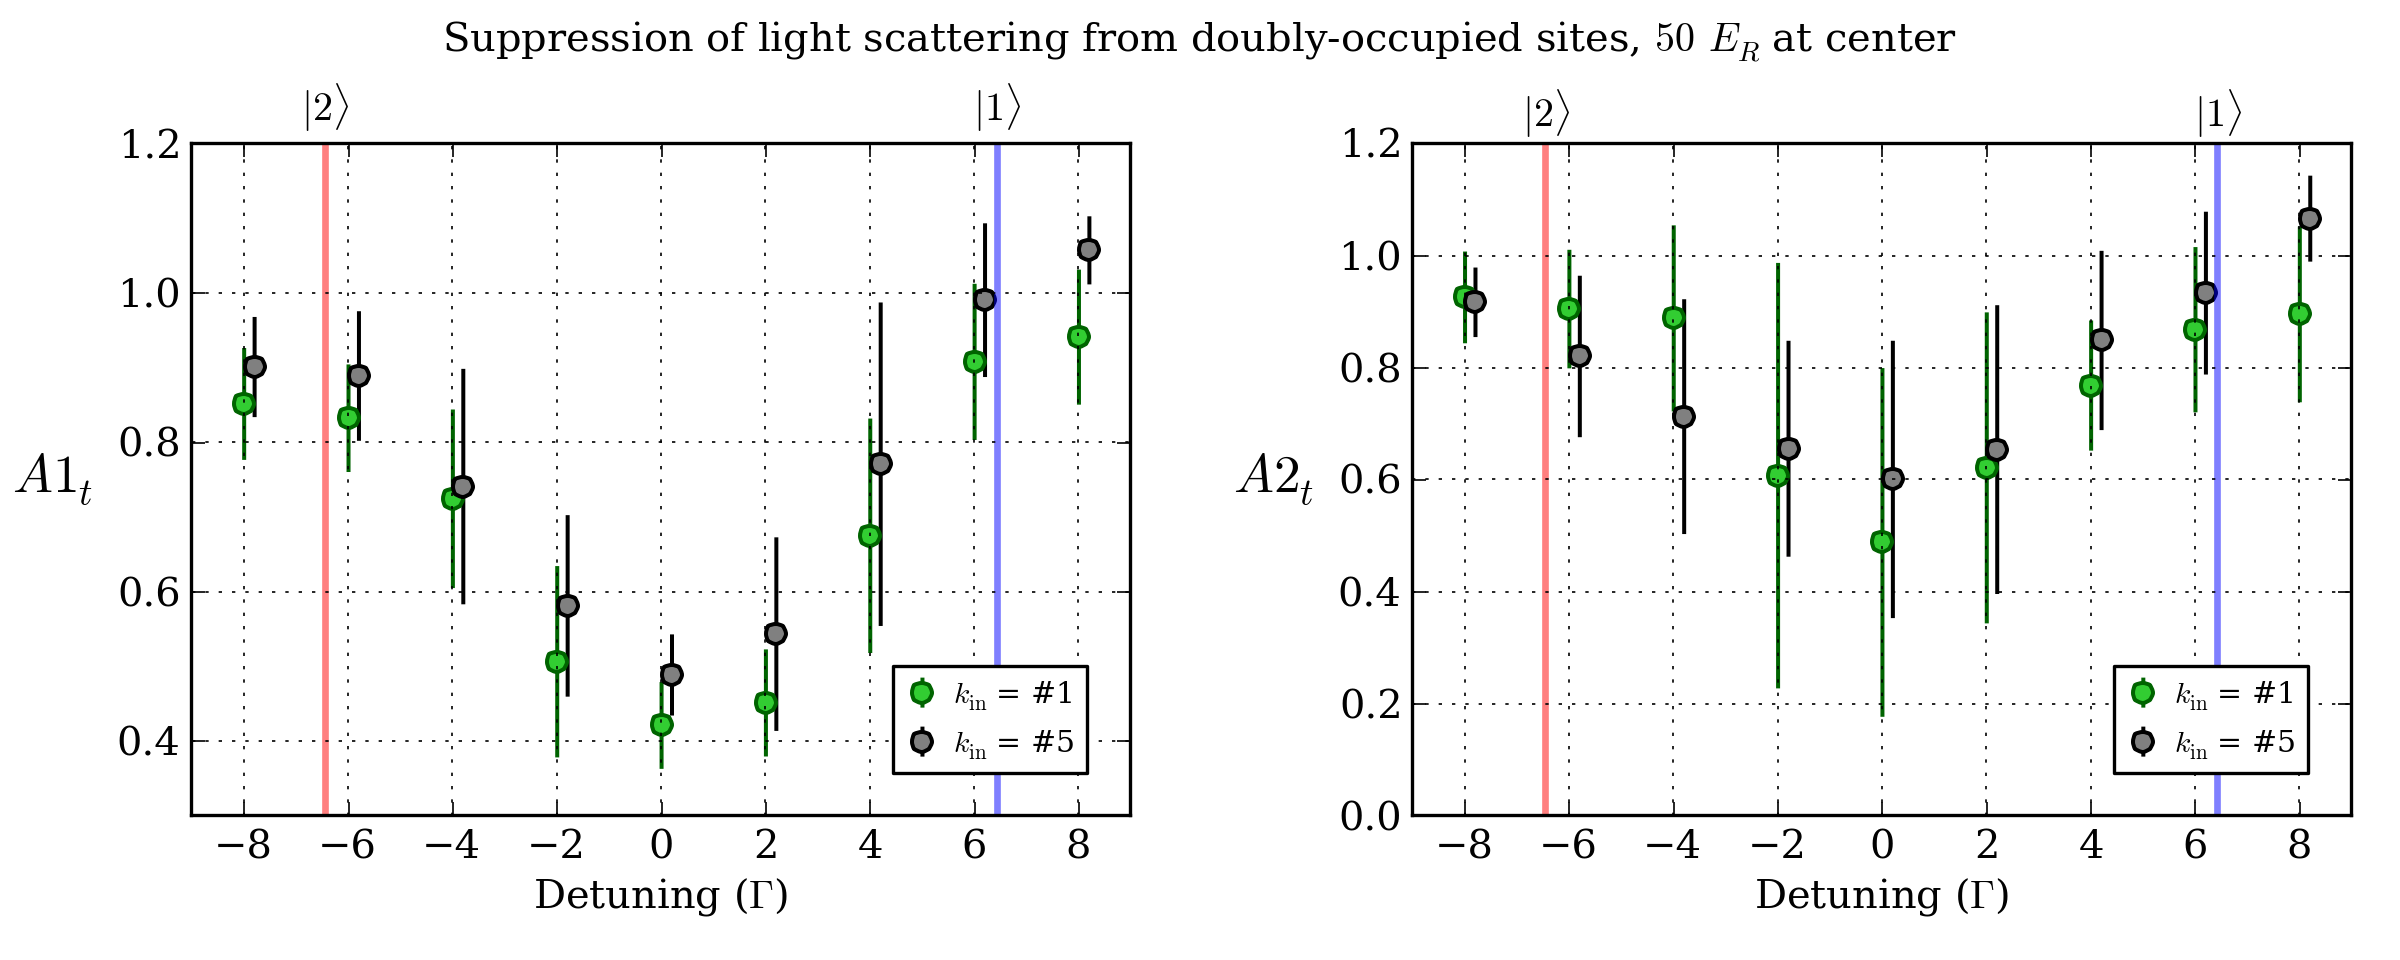
\includegraphics[width=\textwidth]{../Ut_Comp/suppress_Figure_Fancy.png}
\caption[Suppression of light scattering from doubly-occupied sites.]{\small
Suppression of light scattering from doubly-occupied sites.  The suppression is
strongest for a detuning in between the two hyperfine states.  This is the same
detuning used in the spin sensitive \hhh\ Bragg scattering.}
\label{fig:lightsuppress} 
\end{figure}
For reference we show the Debye-Waller factors for the several directions,
including $\bv{k}_{in} = $\#1, \#5,  in Fig.~\ref{fig:debyewaller_v0}
\begin{figure} \centering
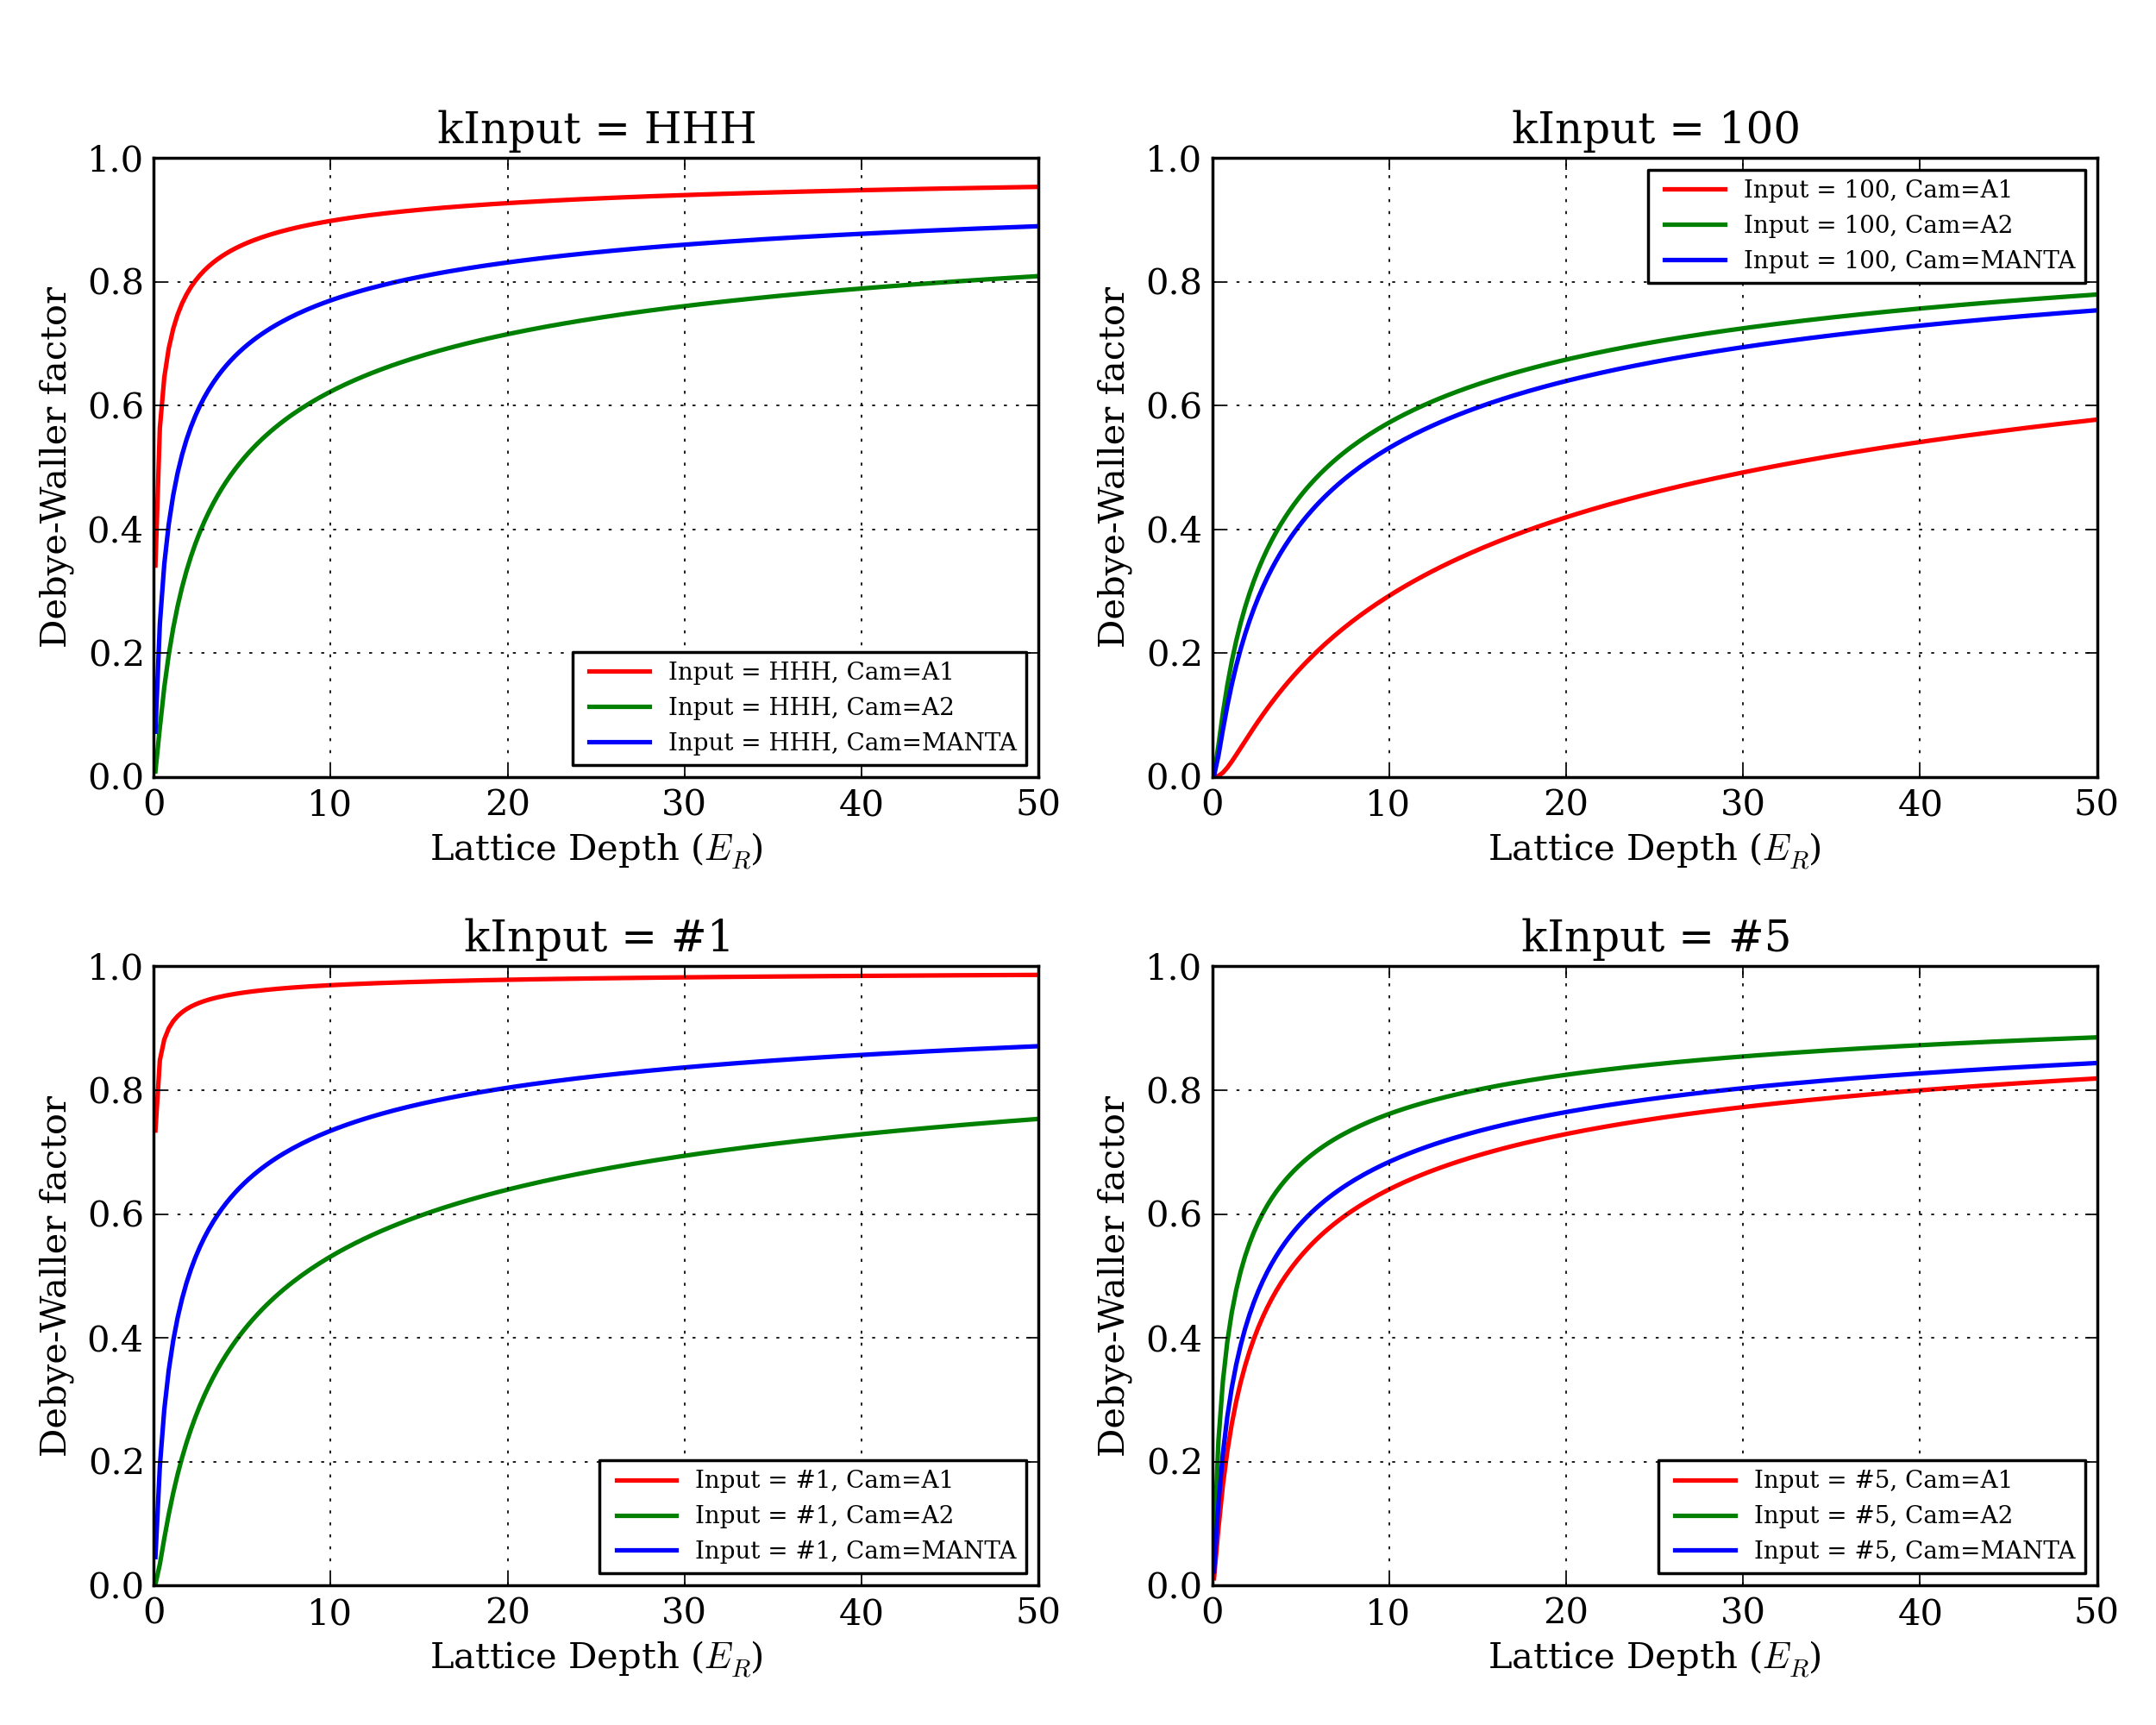
\includegraphics[width=\textwidth]{../Ut_Comp/DWv0_plot.png}
\caption[Debye-Waller factor for various inputs as a function of lattice depth.]{\small Debye-Waller factor for various inputs as a function of lattice depth.}
\label{fig:debyewaller_v0} 
\end{figure}

 
 
\subsection{Disclaimer and what's next}
\label{sec:disclaimer}

In between taking the doublon data and the Bragg data we had to recalibrate the
lattice beams.  This resulted in a correction so that the doublon data is not
at $7\,E_{R}$ lattice depth  as we intended, but more likely at lattice depths
of $7.5, 7.5, 8.5,\,E_{R}$ in each of the three directions.   Our aim right now
is to take more Bragg data in order to reduce the size of the error bars in the
$U/t$ curve.   After we are done with this, we want to follow up with the
doublon data and using the capability of measuring the double-occupancy
in-situ. 



%\cite{PhysRevA.86.023606}

 

\bibliographystyle{osa}
\bibliography{lattice_lda}

\end{document}




